\section{What survives}
\label{sec:survives}

The MoE-matched comparison shows DG's advantage is concentrated at
serial mode. DG wins at every practical output length. The five
conditions that define the regime where block diffusion is the right
choice are:
\begin{enumerate}[nosep]
  \item Output length $\geq 48$ tokens (DG crossover in serial).
  \item Batch-1 by requirement: tenant isolation, interactivity, or
    serial chain structure.
  \item Completeness is validated against a schema.
  \item The quality floor exceeds what the AR model delivers.
  \item A \dgWeights\,GB resident footprint is acceptable.
\end{enumerate}

\paragraph{Why serial investigation chains are where the staircase wins.}

A security operations centre receives an alert, looks up threat
intelligence, cross-references internal logs, and drills into the next
layer. Each hop blocks on the previous; concurrency is 1 by
construction. Against the AR-30B anchor, DG is $2.3\times$ faster per
hop --- 945\,ms vs 419\,ms --- a cross-harness figure. Only the dense
AR-3B was run through the chain harness, at 808\,ms/hop, $1.9\times$
against DG; Figure~\ref{fig:chains} shows that pairing. What the
figure establishes is the \emph{shape}: neither the per-hop cost nor
DG's tail penalty grows with depth. The gap widens in absolute terms
as hops accumulate, at eight hops, the difference between three
seconds and eight seconds is the difference between catching an
intruder in the act and finding the trail gone cold.

A multi-turn code correction chain on HumanEval
(Appendix~\ref{app:humaneval}, Table~\ref{tab:chain}) confirms this
with variable-content rounds (generate $\to$ execute $\to$ fix):
DG's per-round p50 stays flat at 287--305\,ms ($+6\%$), while AR's
grows from 511 to 620\,ms ($+21\%$) as fix prompts accumulate
context. The staircase shape holds across hops that do different
things, not just repeated identical calls.

\begin{figure}[ht!]
\centering
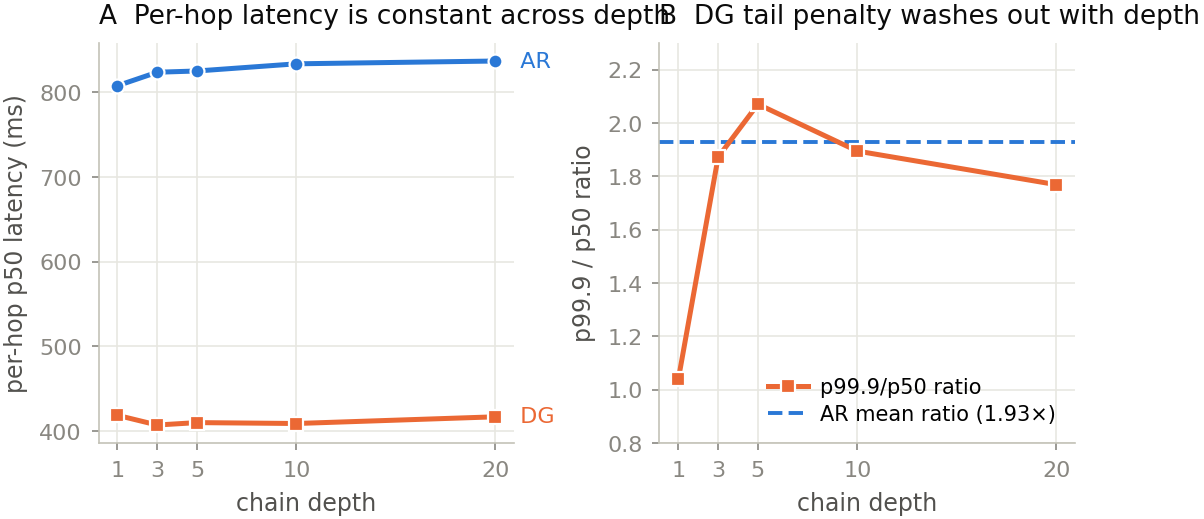
\includegraphics[width=\linewidth]{figures/fig10_usecase_chains.png}
\caption{Serial investigation chains. \textbf{A:} per-hop p50 is
constant across depth, the staircase doesn't steepen. \textbf{B:}
the AR/DG latency ratio at p99.9 climbs from $1.04\times$ at one hop to
$2.07\times$ at five, settling near the median ratio
($1.77$--$1.89\times$) by 10--20 hops. DG's fat tail almost erases its
advantage on a single hop, but independent hops average out, so the
longer the chain the more of its median advantage DG keeps. Note the
arm: this is the dense AR-3B at 808\,ms/hop, hence $1.9\times$ here
against the $2.3\times$ in the text, which is the AR-30B anchor (BGL,
$n{=}100$ chains per depth, $K{=}8$).}
\label{fig:chains}
\end{figure}

\paragraph{What happens when a deadline expires mid-generation?}

A FATAL log line arrives mid-stream. DG's bounded service time and
complete-canvas guarantee make it suitable for priority preemption: a
preempted request returns a valid record, not a truncated one. AR
model, interrupted mid-generation, returns half a JSON object,
syntactically invalid, unusable downstream. In a system that must
decide whether to page an on-call engineer at 3\,a.m., the difference
between a complete record and a truncated one is the difference
between an actionable alert and a false negative.

The $K$ knob is DG's emergency brake: when a deadline tightens, drop
$K$ from 8 to 4 and the model still fills every field, just with
slightly less precision, instead of cutting the JSON in half
mid-key. AR has no counterpart; its only response to a deadline is
truncation. The completeness guarantee holds only above the canvas
length; below $L{=}128$ DG's schema validity collapses to
\dgValidTwentyEight\% against AR's \arValidTwentyEight\%
(Appendix~\ref{app:quality}). Graceful degradation is a property of
the \emph{time} budget, not the output-length budget.

\paragraph{Why autonomous driving is batch-1 by construction.}

One vehicle, one scene, one decision. There is no batching a braking
decision, the car either processes the scene or it doesn't. The
$K$ knob is a per-request quality slider: drop $K$ to meet a tightened
deadline without truncating output. Output is long, multi-object
scene description, predicted trajectories, which is exactly where
the staircase advantage is largest.

\paragraph{Why algorithmic trading rewards long chains.}

A serial chain with a 1--5\,s market reaction window. At eight or more
hops, DG's staircase advantage provides faster end-to-end analysis.
The taxi fare compounds; the subway fare doesn't.

\paragraph{Why wide schemas favour joint denoising.}

DG's joint-canvas denoising treats all fields as one structured
object. Across schema widths from 12 to 100 fields, DG's latency
advantage held between $1.8\times$ and $3.0\times$
(Figure~\ref{fig:schema}; measured against the dense AR-3B baseline,
not AR-30B).

\begin{figure}[ht!]
\centering
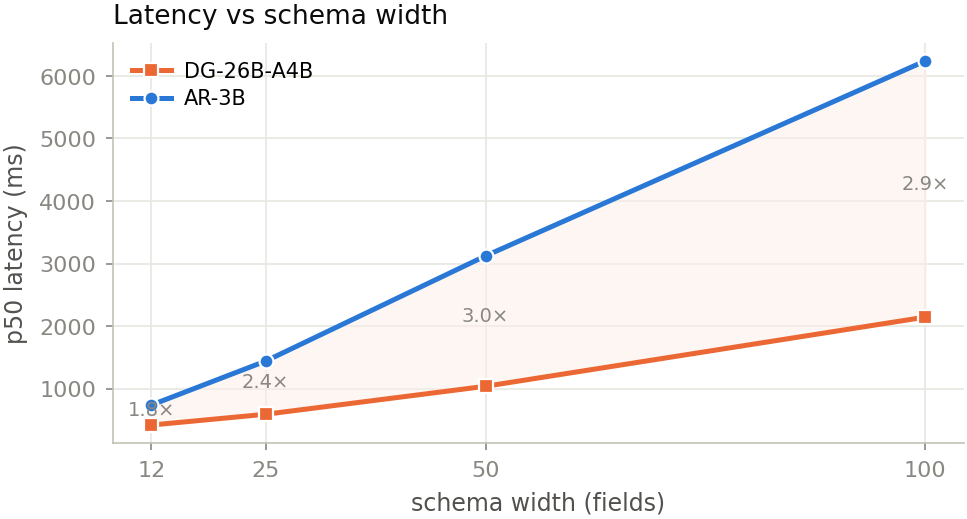
\includegraphics[width=0.85\linewidth]{figures/fig11_usecase_schema.png}
\caption{Latency vs schema width (BGL, $n{=}200$; AR arm is the dense
AR-3B). DG's advantage \emph{rises} with width, from $1.8\times$ at 12
fields to $2.9$--$3.0\times$ at 50--100 fields, because AR pays per
field while DG pays per canvas, though at 100 fields the output no
longer fits one canvas, so DG climbs to $\sim$2{,}140\,ms too and the
ratio stops growing.}
\label{fig:schema}
\end{figure}

\paragraph{Anytime escalation: input-dependent latency.}

The $K$ knob need not be fixed. A cascade runs DG at $K{=}2$ first
(200\,ms), checks whether the output is complete (all structural
fields filled), and escalates only incomplete records to $K{=}8$
(376\,ms). AR has no equivalent: it cannot inspect partial output
quality mid-generation and decide whether to continue. AR's early
stopping is binary --- the model either emits EOS or it doesn't ---
while DG's is graduated across $K$ steps. This makes DG's latency
\emph{input-dependent} in a way AR structurally cannot be.

We measured the cascade on BGL ($n{=}200$, canvas$=256$): 29.5\% of
records resolved at $K{=}2$; the remaining 70.5\% escalated to
$K{=}8$. The cascade F1 was 0.848 (a drop of 0.005 vs fixed $K{=}8$),
but the average latency was 465\,ms --- \emph{slower} than fixed
$K{=}8$ (376\,ms), because the $K{=}2$ pass adds overhead that is
only amortised if most inputs resolve early. On this task, 70\% of
inputs need $K{=}8$, so the cascade does not save latency. The
structural property (input-dependent latency is possible) is
confirmed; the practical benefit is task-dependent and favours tasks
where easy inputs dominate.

\paragraph{Where diffusion does not win.}

High-rate log streams favour AR's batching advantage. Tail-sensitive
single-stream workloads with strict p99 SLAs are hurt by DG's
max/median ratio. And any workload that can batch favours AR
regardless of output length.

\paragraph{Where diffusion fails.}

Six hypotheses about diffusion's structural advantages were tested and
refuted; see Appendix~\ref{app:refuted}. Three of the six, the
perturbation, refinement and bounded-deadline probes, were run on a
second diffusion model, \LLaDA\ (LLaDA-8B-Instruct), against the dense
AR-3B, because they predate the DiffusionGemma arm. We report them
because the hypotheses concern block diffusion as a class, but they
are not measurements of DG. The most instructive failures: bidirectional
attention propagates input noise in both directions, making the
diffusion arm \emph{less} robust to perturbation than AR in all ten
tested categories. Joint denoising should preserve suffix tokens by
construction, but AR trivially regenerates the whole record from the
prompt, that probe is DG (Appendix~\ref{app:refuted}). And selective
re-masking gains a small F1 improvement over three rounds, but still
trails AR after a single pass. These failures
define where it stops working: block diffusion's advantage is in
\emph{latency shape at long output}, not in robustness, infilling, or
iterative refinement.

